\documentclass{report}
\usepackage {array}

\usepackage{graphicx}
\graphicspath{ {../img/} }

\usepackage{float}

\newcommand{\nonterm}[1]{\langle #1 \rangle}
\newcommand{\term}[1]{\texttt{#1}}

\title {ProgettoLC parte4parz Gruppo 8 Relazione}
\author{Di Benedetto Gianluca \\ Lattaruolo Andrea \\ Riccardi Brian}
\date{}


\begin{document}
\maketitle
\tableofcontents

\chapter {Descrizione del linguaggio}

\section {Struttura lessicale}

\begin {itemize}
    \item Identificatori e letterali sono i classici definiti da BNFC, con l'unica eccezione per i booleani
    a cui vengono associate le keyword \texttt{false} e \texttt{true}.
    
    \item Le keyword riservate sono:
    \begin{center}
    \begin{tabular}{*{5}{>{\ttfamily}c}}
        bool &  break & char  & const  & continue    \\
        do   &  else  & false & for    & if          \\
        in   &  inout & int   & out    & param       \\
        proc &  real  & ref   & return & string      \\
        then &  true  & var   & void   & while

    \end{tabular}
    \end{center}
    \term{out} viene riservato per utilizzi futuri

    \item I simboli riservati sono:
    \begin{center}
    \begin{tabular}{*{7}{>{\ttfamily}c}}
        !    &  !=   &  \%  &  \%=  &  \&  &  \&\&  &  (    \\
        )    &  *    &  *=  &   +   &  ++  &    ,   &  -    \\
        --   &  -=   &  ..  &   /   &  /=  &    :   &  ;    \\
        <    &  <=   &  ==  &   >   &  >=  &    [   &  ]    \\
        \^{} & \^{}= &  \{  &  \}   &  ||

    \end{tabular}
    \end{center}
    \texttt{++} e \texttt{--} sono stati riservati per utilizzi futuri

    \item I commenti single-line vengono identificati da \texttt{//}, mentre
    i multi-line sono racchiusi tra \texttt{/*} e \texttt{*/}

\end {itemize}

\section {Struttura sintattica}

\begin{itemize}
    \item Un programma è una lista di dichiarazioni.
    
    \item Una dichiarazione di una lista di costanti inizia con la keyword
        \texttt{param} e segue con una lista non vuota di inizializzazioni
        della forma $$\nonterm{Ident} \term{:} \nonterm{Type} \term{=} \nonterm{RExp}$$ separate da \texttt{,}
        e terminate da \texttt{;}

    \item Una dichiarazione di una lista di variabili inizia con la keyword
        \texttt{var} e segue con una lista non vuota di elementi della forma
        $$\nonterm{Ident} \term{:} \nonterm{Type}$$ oppure $$\nonterm{Ident} \term{:} \nonterm{Type} \term{=} \nonterm{RExp}$$,
        separati da \texttt{,} e terminata da \texttt{;}

    \item Una dichiarazione di funzione inizia con la keyword \texttt{proc} seguita da
        $$\nonterm{Ident} \term{(} \nonterm{FormList} \term{)} \term{:} \nonterm{Type} \nonterm{Block}$$\\
        La lista di parametri formali $\nonterm{FormList}$ è una lista possibilmente vuota
        di elementi della forma $$\nonterm{Intent} \nonterm{Ident} \term{:} \nonterm{Type}$$ separati
        da \texttt{,}

    \item Un tipo ha la seguente struttura
        \begin{center}
        \begin{tabular}{l c l}
        $\nonterm{Type}$        &   $::=$   &   $\nonterm{Compound} \nonterm{Basic}$                        \\
        $\nonterm{Compound}$    &   $::=$   &   $\epsilon$                                                  \\
                                &    $|$    &   $\term{[ } \nonterm{RExp} \term{ ]} \nonterm{Compound}$     \\
                                &    $|$    &   $\term{\{ } \nonterm{RExp} \term{ \}} \nonterm{Compound}$   \\
                                &    $|$    &   $\term{* } \nonterm{Compound}$                              \\
        $\nonterm{Basic}$       &   $::=$   &   $\term{bool}$                                               \\
                                &    $|$    &   $\term{char}$                                               \\
                                &    $|$    &   $\term{int}$                                                \\
                                &    $|$    &   $\term{real}$                                               \\
                                &    $|$    &   $\term{string}$                                             \\
                                &    $|$    &   $\term{void}$

        \end{tabular}
        \end{center}

    \item Un intent (modalità di passaggio dei parametri) ha la seguente struttura
        \begin{flushleft}
        \begin{tabular}{ l c l }
        $\nonterm{Intent}$      &   $::=$   &   $\term{in}$                                             \\
                                &    $|$    &   $\term{inout}$                                          \\
                                &    $|$    &   $\term{ref}$                                            \\
                                &    $|$    &   $\term{const in}$                                       \\
                                &    $|$    &   $\term{const ref}$                                      \\
                                &    $|$    &   $\epsilon$

        \end{tabular}
        \end{flushleft}

    \item Un blocco ha forma $\nonterm{Block} ::= \term{\{  } \nonterm{DeclList} \nonterm{StmList} \term{  \}}$
        dove le liste di dichiarazioni e statement possono essere vuote

    \item Una r-espressione ha forma
        \begin{flushleft}
        \begin{tabular}{l c l}
        $\nonterm{RExp}$    &   $::=$   &   $\nonterm{RExp} \nonterm{BinOp} \nonterm{RExp}$             \\
                            &    $|$    &   $\term{! } \nonterm{RExp}$                                  \\
                            &    $|$    &   $\term{\& } \nonterm{RExp}$                                 \\
                            &    $|$    &   $\nonterm{SignOp} \nonterm{RExp}$                           \\
                            &    $|$    &   $\nonterm{LExp}$                                            \\
                            &    $|$    &   $\term{[  } \nonterm{RExpList} \term{  ]}$                  \\
                            &    $|$    &   $\nonterm{Ident} \term{ ( } \nonterm{RExpList} \term{ ) }$  \\
                            &    $|$    &   $\nonterm{Literal}$

        \end{tabular}
        \end{flushleft}

        \begin{flushleft}
        \begin{tabular}{*{5}c}
        $\nonterm{SignOp}$  &   $::=$   &   $\term{+}$                                           
                            &    $|$    &   $\term{-}$   

        \end{tabular}
        \end{flushleft}

        \begin{flushleft}
        \begin{tabular}{*{15}c}
        $\nonterm{BinOp}$   &   $::=$   &   $\term{||}$
                            &    $|$    &   $\term{\&\&}$
                            &    $|$    &   $\term{+}$
                            &    $|$    &   $\term{-}$
                            &    $|$    &   $\term{*}$
                            &    $|$    &   $\term{/}$
                            &    $|$    &   $\term{\%}$         \\
                            &    $|$    &   $\term{\^{}}$
                            &    $|$    &   $\term{<}$
                            &    $|$    &   $\term{<=}$
                            &    $|$    &   $\term{==}$
                            &    $|$    &   $\term{!=}$
                            &    $|$    &   $\term{>=}$
                            &    $|$    &   $\term{>}$

        \end{tabular}
        \end{flushleft}

        \begin{flushleft}
        \begin{tabular}{*{3}c}
        $\nonterm{Range}$   &   $::=$   &   $\term{\{ } \nonterm{RExp} \term{ .. } \nonterm{RExp} \term{ \}}$   

        \end{tabular}
        \end{flushleft}

    \item Una l-espressione ha forma
        \begin{flushleft}
        \begin{tabular}{l c l}
        $\nonterm{LExp}$    &   $::=$   &   $\term{* } \nonterm{LExp}$                                  \\
                            &    $|$    &   $\nonterm{LExp} \term{ [ } \nonterm{RExp} \term{ ]}$        \\
                            &    $|$    &   $\nonterm{Ident}$

        \end{tabular}
        \end{flushleft}

    \item Uno statement ha forma
        \begin{flushleft}
        \begin{tabular}{l c l}
        $\nonterm{Stm}$     &   $::=$   &   $\nonterm{Block}$                                                                   \\
                            &    $|$    &   $\nonterm{Ident} \term{ ( } \nonterm{RExpList} \term{ ) } \term{ ;}$                \\
                            &    $|$    &   $\nonterm{LExp} \nonterm{AssignOp} \nonterm{RExp} \term{ ;}$                        \\
                        %   &    $|$    &   $\nonterm{LExp} \term{;}$                                                           \\
                            &    $|$    &   $\term{if } \nonterm{RExp} \term{ then } \nonterm{Stm}$                             \\
                            &    $|$    &   $\term{if } \nonterm{RExp} \nonterm{Block}$                                         \\
                            &    $|$    &   $\term{if } \nonterm{RExp} \term{ then } \nonterm{Stm} \term{ else } \nonterm{Stm}$ \\
                            &    $|$    &   $\term{if } \nonterm{RExp} \nonterm{Block} \term{ else } \nonterm{Stm}$             \\
                            &    $|$    &   $\term{while } \nonterm{RExp} \term{ do } \nonterm{Stm}$                            \\
                            &    $|$    &   $\term{while } \nonterm{RExp} \nonterm{Block}$                                      \\
                            &    $|$    &   $\term{do } \nonterm{Stm} \term{ while } \nonterm{RExp} \term{ ;}$                  \\
                            &    $|$    &   $\term{for } \nonterm{Ident} \term{ in } \nonterm{Range} \term{ do } \nonterm{Stm}$ \\
                            &    $|$    &   $\term{for } \nonterm{Ident} \term{ in } \nonterm{Range} \nonterm{Block}$           \\
                            &    $|$    &   $\nonterm{Jump} \term{ ;}$                                                          \\
        \                   &    \      &   \                                                                                   \\
        $\nonterm{Jump}$    &   $::=$   &   $\term{break}$                                                                      \\
                            &    $|$    &   $\term{continue}$                                                                   \\
                            &    $|$    &   $\term{return}$                                                                     \\
                            &    $|$    &   $\term{return } \nonterm{RExp}$

        \end{tabular}
        \end{flushleft}

        \begin{flushleft}
        \begin{tabular}{*{15}c}
        $\nonterm{AssignOp}$    &   $::=$   &   $\term{=}$                                           
                                &    $|$    &   $\term{+=}$                                          
                                &    $|$    &   $\term{-=}$                                        
                                &    $|$    &   $\term{*=}$                                          
                                &    $|$    &   $\term{/=}$                                     
                                &    $|$    &   $\term{\%=}$                                    
                                &    $|$    &   $\term{\^{}=}$
        \end{tabular}
        \end{flushleft}

    \item La seguente tabella descrive le precedenze e associatività dei vari operatori (in ordine crescente di precedenza)
        \begin{center}
        \begin{tabular}{ | c | c | }
            \hline
            \textbf{Simbolo}                        &       \textbf{Associatività}  \\
            \hline
            \term{||}                               &       Sinistra                \\
            \hline
            \term{\&\&}                             &       Sinistra                \\
            \hline
            \term{==} \term{!=}                     &       Non associa             \\
            \hline
            \term{<} \term{<=} \term{>=} \term{>}   &       Non associa             \\
            \hline
            \term{+} \term{-}                       &       Sinistra                \\
            \hline
            \term{*} \term{/} \term{\%}             &       Sinistra                \\
            \hline
            \term{!} \term{+unary} \term{-unary}    &       Destra                  \\
            \hline
            \term{\^{}}                             &       Destra                  \\
            \hline
        \end{tabular}
        \end{center}

\end{itemize}


\section {Vincoli semantici}

\begin {itemize}
    \item La compatibilità tra tipi prevede:
    \begin{itemize}
        \item il tipo \term{bool} compatibile con i tipi \term{char}, \term{int} e \term{real}
        \item il tipo \term{char} compatibile con i tipi \term{int} e \term{real}
        \item il tipo \term{int} compatibile con il tipo \term{real}
        \item se $\tau_1$ è compatibile con $\tau_2$ allora $[n]\tau_1$ è compatibile con $[n]\tau_2$;
            array di dimensioni diverse non son compatibili tra loro.
        \item i puntatori non sono compatibili tra loro.

    \end{itemize}

    \item Per alcuni operatori è presente l'overloading, in particolare:
        \begin{center}
        \begin{tabular}{ | c | c | }
            \hline
            \textbf{Simbolo}                        &       \textbf{Tipo}                                               \\
            \hline
            \term{||} \term{\&\&}                   &       $\term{bool} \times \term{bool} \rightarrow \term{bool}$    \\
            \hline
            \term{==} \term{!=} \term{<}            &       $\tau \times \tau \rightarrow \term{bool}$                  \\
            \term{<=} \term{>=} \term{>}            &       $\tau \in \{\term{bool}, \term{char}, \term{int}, \term{real}, \term{string}, pointer\footnotemark\}$    \\
            \hline
            \term{+} \term{-}                       &       $\tau \times \tau \rightarrow \tau$                         \\
            \term{*} \term{/}                       &       $\tau \in \{\term{int}, \term{real}\}$                      \\
            \hline
            \term{\%}                               &       $\term{int} \times \term{int} \rightarrow \term{int}$       \\
            \hline
            \term{!}                                &       $\term{bool} \rightarrow \term{bool}$                       \\
            \hline 
            \term{+unary} \term{-unary}             &       $\tau \rightarrow \tau$                                     \\
                                                    &       $\tau \in \{\term{int}, \term{real}\}$                      \\
            \hline
            \term{\^{}}                             &       $\tau \times \term{int} \rightarrow \tau$                   \\
                                                    &       $\tau \in \{\term{int}, \term{real}\}$                      \\
            \hline
        \end{tabular}
        \end{center}
        \footnotetext{Ovviamente intesi puntatori dello stesso tipo.}

    Le guardie di costrutti di iterazione indeterminata e condizionali devono avere tipo \term{bool}

    \item Le modalità di passaggio dei parametri previste sono: \term{in} (valore),
    \term{inout} (valore-risultato), \term{ref} (riferimento),
    \term{const in} (costante-valore), \term{const ref} (costante-riferimento) con i
    seguenti vincoli e semantica:
    \begin{description}
        \item[in:] il parametro attuale deve essere compatibile con il formale;
            viene effettuata una copia prima del passaggio
        \item[inout:] il formale e l'attuale devono avere lo stesso tipo, l'attuale
            deve essere una l-espressione mutabile e il formale deve essere assegnato
            in ogni percorso di esecuzione; viene passato un riferimento all'attuale,
            viene eseguita una copia locale e al termine dell'esecuzione della funzione,
            il formale viene ri-copiato nell'attuale
        \item[ref:] il formale e l'attuale devono avere lo stesso tipo e l'attuale deve
            essere una l-espressione mutabile; viene passato un riferimento dell'attuale
        \item[const in:] come \term{in} e il formale viene reso immutabile
        \item[const ref:] come \term{ref} e il formale viene reso immutabile

    \end{description}
    L'intento $\epsilon$ viene considerato \term{in}.

    \item I namespace di variabili, costanti e funzioni è lo stesso: la ridefinizione di un nome
    è permessa solo all'interno di un nuovo blocco.

    Il tipo \term{void} \textbf{non} può essere utilizzato nella dichiarazione di una variabile,
    costante o di un parametro formale.

    Le variabili possono \textbf{non} essere inizializzate esplicitamente, in tal caso
    vengono inizializzate implicitamente nei seguenti modi:
    \begin{itemize}
        \item \term{bool} come \term{false}
        \item \term{char} come \texttt{\textbackslash 0} (ASCII 0)
        \item \term{int} come 0
        \item \term{real} come 0.0
        \item \term{string} come \term{""}
        \item puntatori come \term{nullptr}
        \item array di tipo $[n]\tau$ come array di $n$ valori di default
            per il tipo $\tau$
        
    \end{itemize}

    La dimensione di un array deve essere una r-espressione valutabile a compile-time,
    compatibile con il tipo intero e di valore positivo.

    Le costanti (\term{param}) sono considerate immutabili e definite a compile-time.
    Devono essere inizializzate solo da letterali o da r-espressioni valutabili
    a compile-time.

    Variabili e costanti sono visibili dal punto di dichiarazione fino alla fine
    del blocco, le funzioni sono visibili ovunque nel blocco di dichiarazione
    e nei blocchi al suo interno.

    Le funzioni (non procedure) devono ammettere un return in ogni path di esecuzione
    possibile.

    \item Non è possibile utilizzare l'operatore di referenziazione \term{\&} su una
    l-espressione immutabile.

    \item Le chiamate a funzione (non chiamate a procedura) non possono essere utilizzate come
    statement. Le chiamate a procedura (non chiamate a funzione) non possono essere utilizzate in un
    assegnamento.

    \item Sono presenti i costrutti di iterazione indeterminata \term{while} e
    \term{do-while} con la usuale semantica.

    \item È presente il costrutto di iterazione determinata \texttt{for i in \{s .. e\}~stm}
    con i seguenti vincoli: \texttt{i} viene considerato immutabile nello statement del ciclo,
    dichiarata (non nel blocco di iterazione e quindi ri-dichiarabile al suo interno) di tipo 
    \term{int} e viene incrementato di 1 ad  ogni iterazione; le r-espressioni \texttt{s} 
    ed \texttt{e} devono essere  compatibili con il tipo \term{int}; i limiti del ciclo 
    vengono calcolati solo alla prima guardia e \texttt{i} viene inizializzato con il 
    valore di \texttt{s}; il ciclo termina quando \texttt{i > e}.

    \item \texttt{break} e \texttt{continue} possono essere utilizzati solo all'interno
    di un costrutto di iterazione indeterminata non contenuto in un costrutto di iterazione determinata.

    \item \texttt{return} e \texttt{return e} non possono essere utilizzati all'interno
    di costrutti di iterazione (determinata e non). \texttt{return} può essere utilizzato
    solo all'interno di una procedura. \texttt{e} deve essere compatibile con
    il tipo di ritorno della funzione.

    \item In ogni funzione vengono mantenuti solo gli statement che possono essere raggiunti
    da un qualche path di esecuzione.

    \item Nell'ambiente globale deve essere presente una procedura con signature
        \texttt{proc main():void}.

\end {itemize}

\begin{figure}[H]
\centering
\includegraphics[width = \linewidth]{types}
\caption {Rappresentazione grafica della compatibilità tra tipi.}
\end{figure}

\section {Altre caratteristiche}

\begin{itemize}
    \item Le r-espressioni di inizializzazione per le costanti e le dimensioni degli array
        vengono valutate a compile-time.
    
    \item Le guardie dei costrutti di iterazione indeterminata e dei condizionali vengono valutate
        con short-cut.
    
    \item Le r-espressioni di tipo \term{bool} vengono valutate con short-cut: si è deciso così
        perché una volta implementato lo short-cut per le guardie è immediato implementarlo per
        tutte le espressioni booleane.
    
    \item Negli assegnamenti vengono valutate le l-espressioni prima delle r-espressioni
    
    \item La valutazione delle espressioni e degli argomenti viene effettuata da sinistra verso destra:
        non c'è una ragione precisa per il verso, ma l'idea di avere un ordine ben determinato e non
        casuale permette al programmtore di prevedere più facilmente i side-effect generati dalla
        valutazione.

    \item Sono presenti delle funzioni monomorfe predefinite per la lettura e la scrittura di 
        char, int, real, string. È presente una funzione predefinita dalla signature
        \term{proc outOfBounds(): void} per la gestione di errori a runtime sugli indici di array
        dichiarati checked. È inoltre presente una funzione predefinita per la comparazione
        tra stringhe dalla signature \\\term{proc~stringCmp(string,~int,~string):~bool} che attribuisce
        un valore di verità al confronto tra due stringhe attraverso un determinato operatore
        (specificato dal parametro intero).
        \begin{center}
        \begin{tabular}{ | c | c | }
            \hline
            $n$     &   \textbf{Operatore}  \\
            \hline
            0       &   \term{<}            \\
            \hline
            1       &   \term{<=}           \\
            \hline
            2       &   \term{==}           \\
            \hline
            3       &   \term{!=}           \\
            \hline
            4       &   \term{>=}           \\
            \hline
            5       &   \term{>}            \\
            \hline
            
        \end{tabular}
        \end{center}

    \item La semantica di confronto tra array o puntatori compatibili tra loro prevede il confronto
        del valore numerico dell'indirizzo associato alla base degli array (nel caso di array) o all'indirizzo
        contenuto (nel caso di puntatori).

\end{itemize}

\chapter {Type system}

\begin{figure}
    \centering
    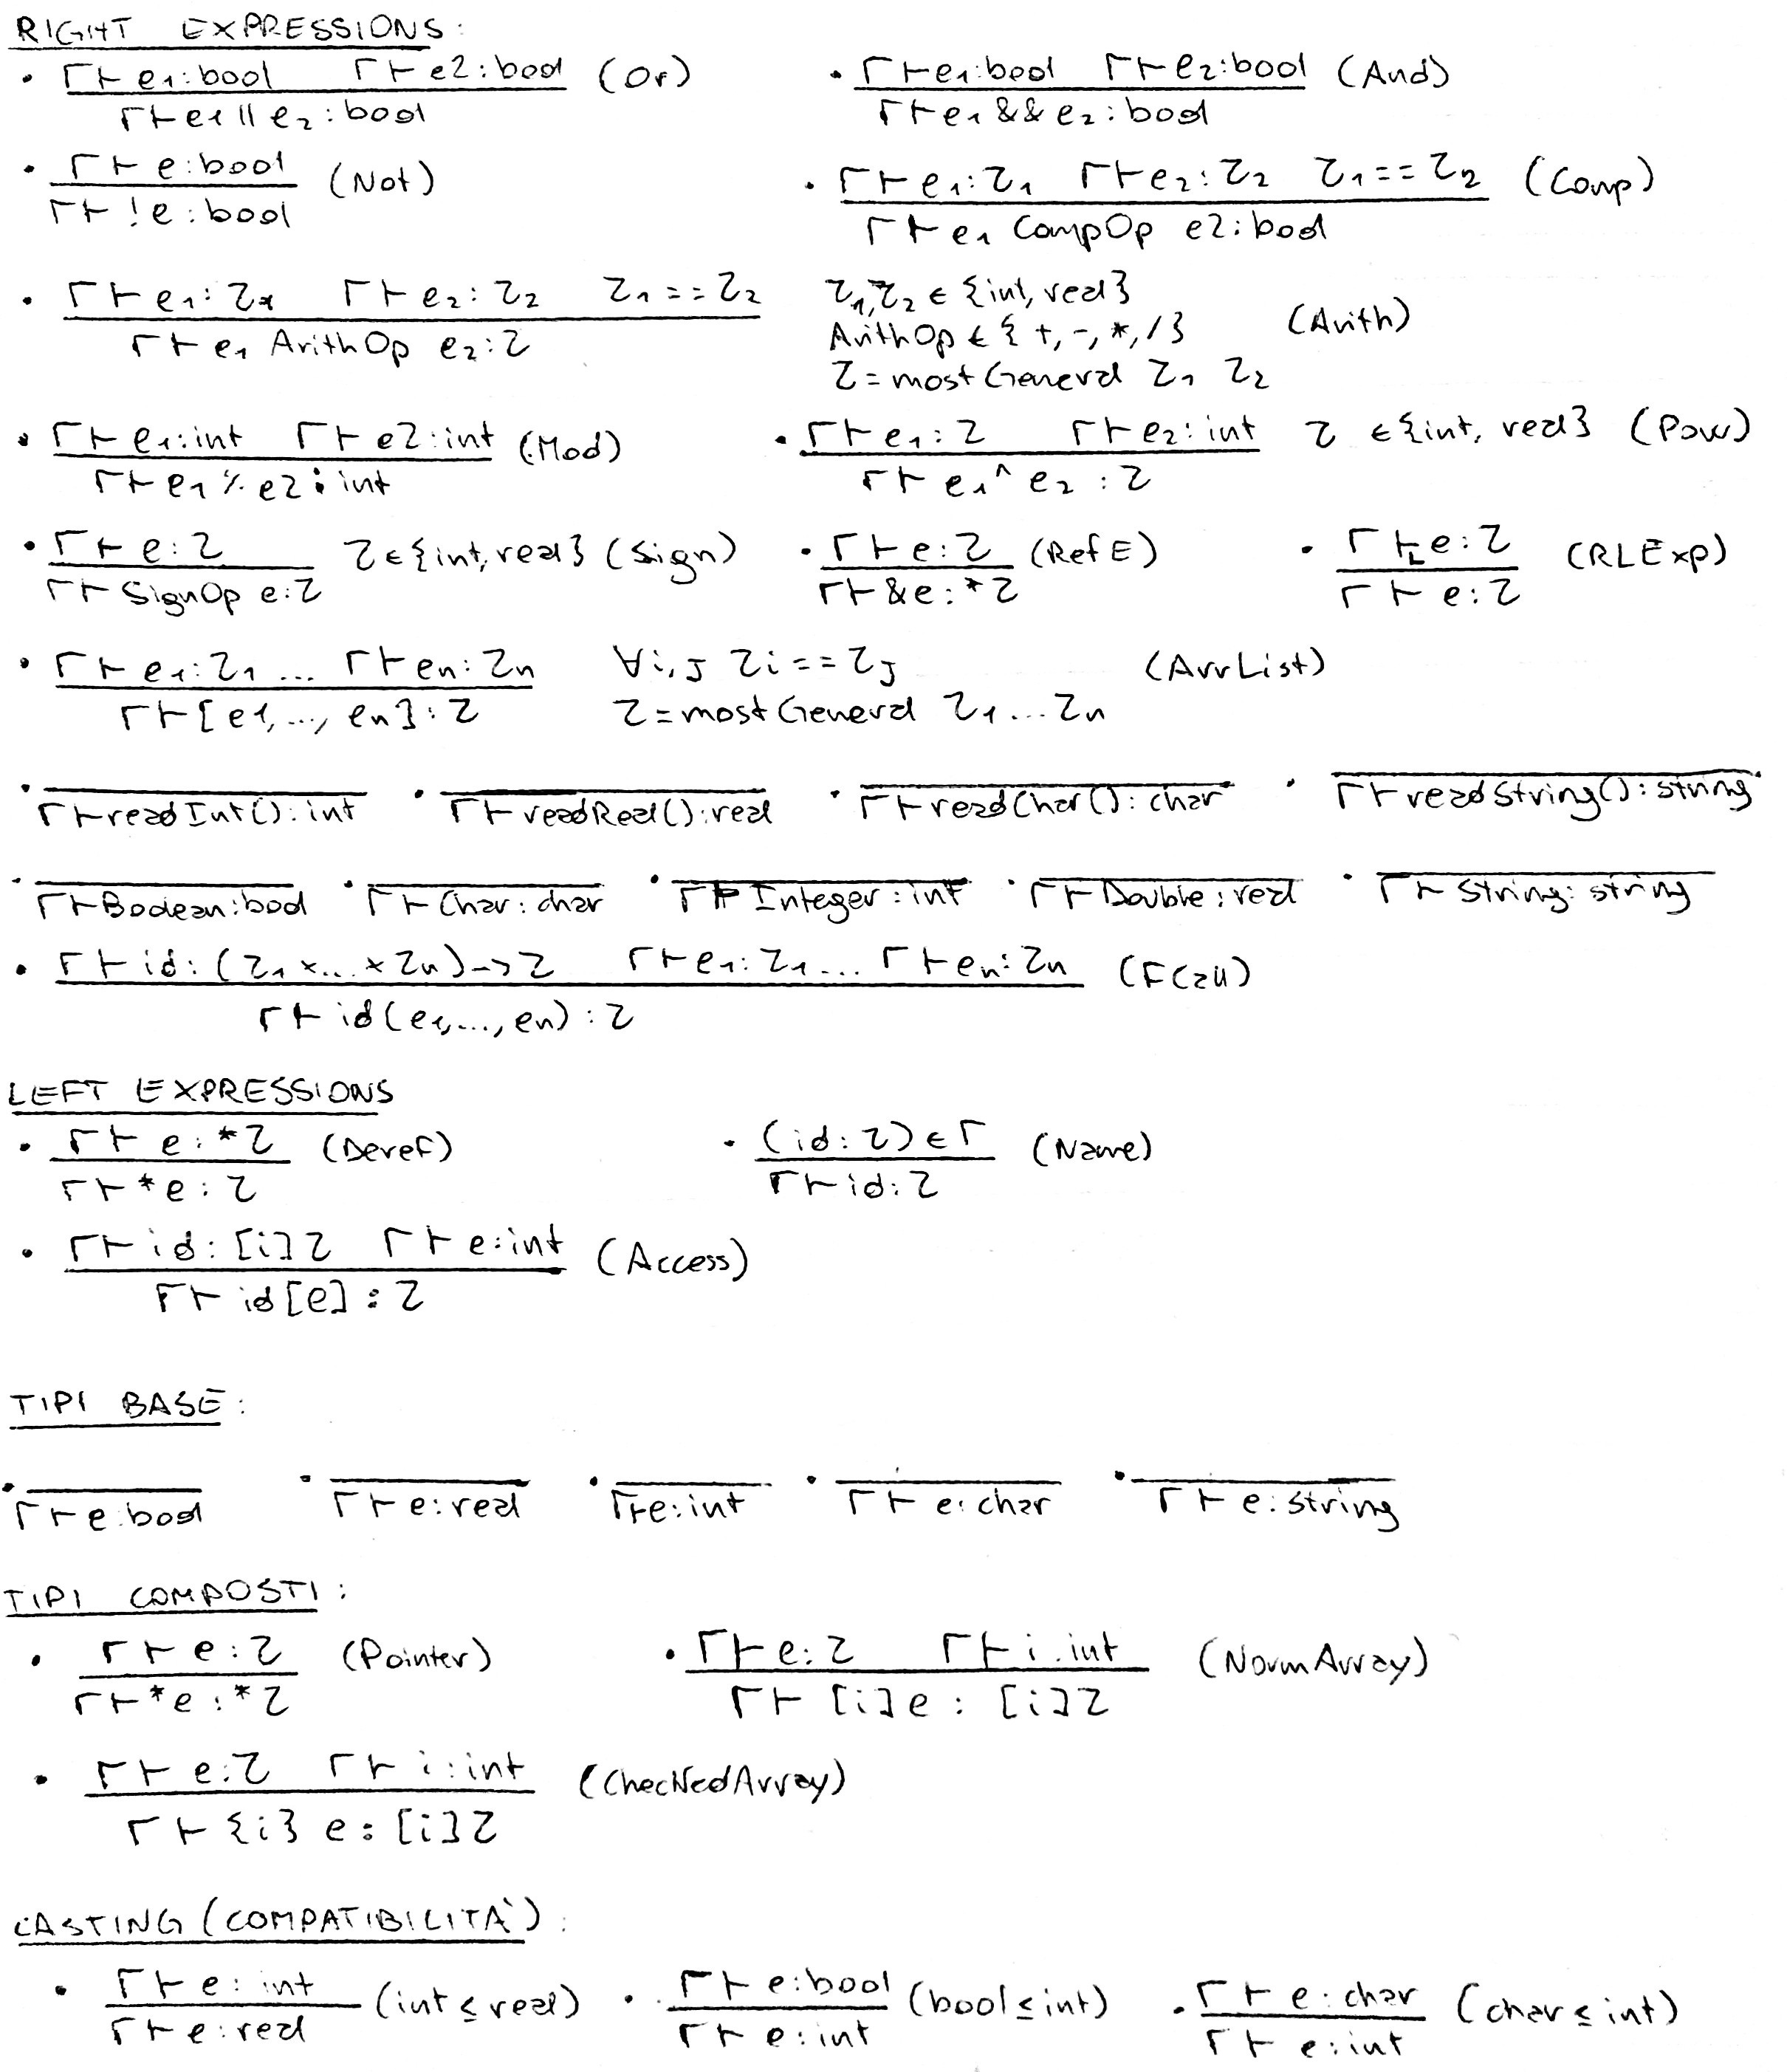
\includegraphics[width = 1.2\linewidth]{typesystem2}
\end{figure}

\begin{figure}
    \centering
    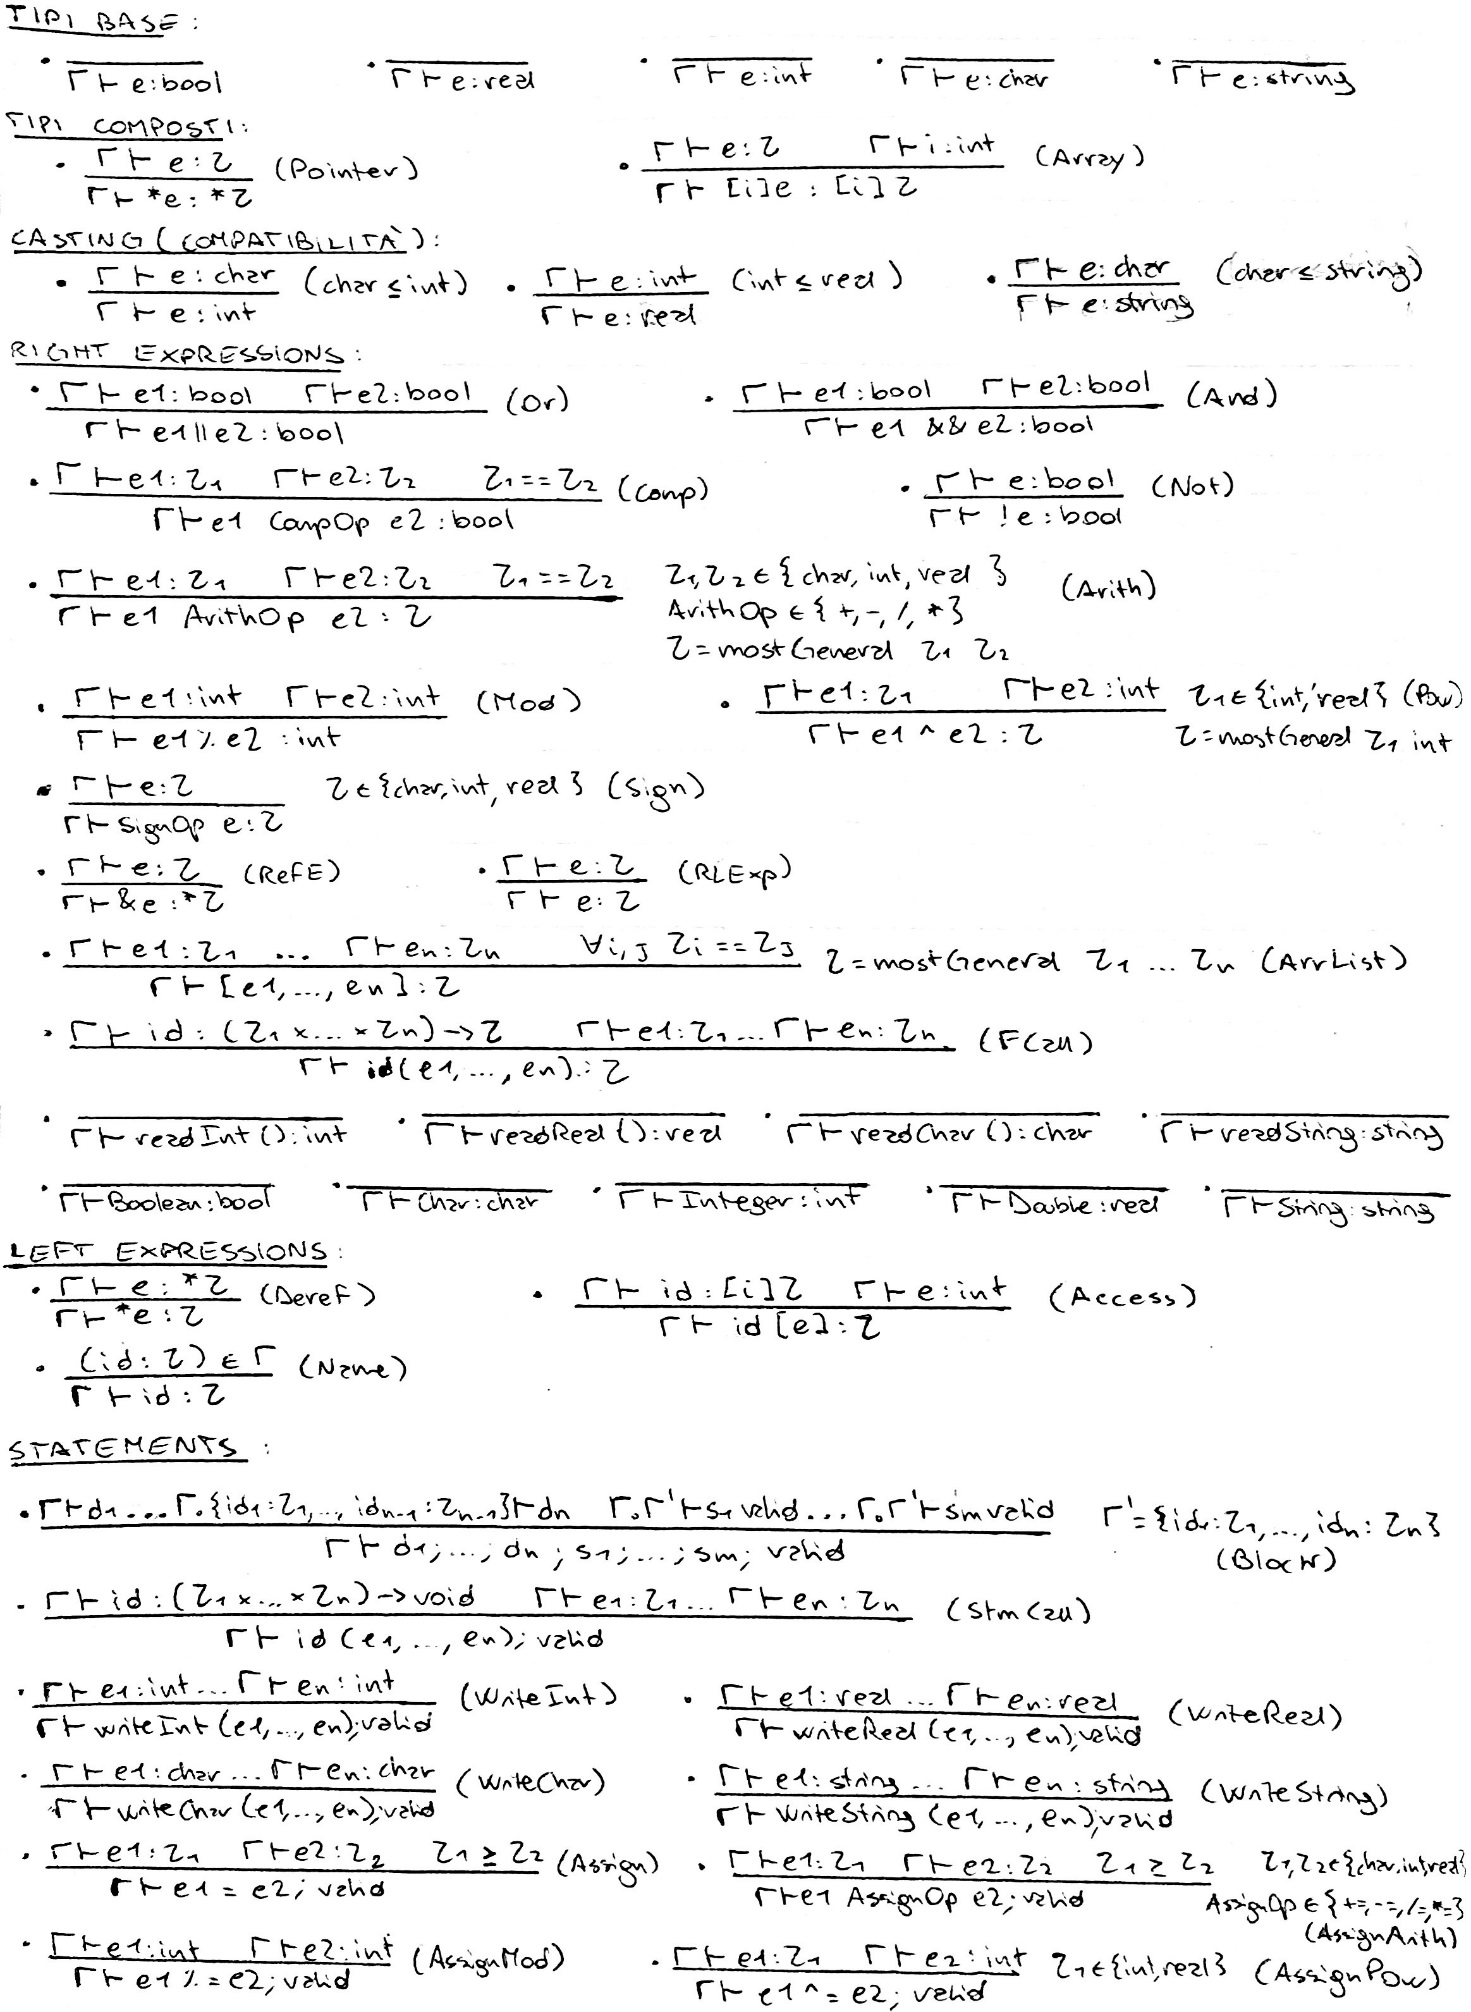
\includegraphics[width = 1.2\linewidth]{typesystem1}
\end{figure}


\chapter {Descrizione del codice e testing}

\section{Struttura del codice}

È stata inizialmente utilizzto BNFC per una prima bozza di Lexer, Parser, tipi di dato per l'AST e 
Prettyprinter delll' AST. Successivamente sono stati ritoccati:
\begin{itemize}
    \item il Lexer, aggiungendo alcune funzioni per recuperare informazioni riguardo i token
    \item il Parser, modificando associatività e precedenza degli operatori, nonché snellendo
        il parser stesso e modificando i dati costruiti dalle produzioni per renderli compatibili con
        le modifiche effettuate ai tipi dell'AST
    \item i tipi di dato dell'AST per permettere il salvataggio dell'informazione della posizione nel codice e
        rendendo i tipi di dato polimorfi per essere ``etichettati'' nella fase di type-checking; sono stati aggiunti
        dei fieldname per recuperare in modo pulito le informazioni necessarie; sono state inoltre definite delle istanze
        Functor per etichettare velocemente i dati in situazioni particolari (si vedano le funzioni \term{set} e \term{coerce});
        sono stati aggiunti un costruttore alle r-espressioni per permettere la conversione implicita di tipo, e dei costruttori
        per il tipo Literal per semplificare la gestione dei valori di default
    \item il Prettyprinter è stato adattato alle modifiche dell'AST
\end{itemize}

Abbiamo quindi definito dei moduli per strutturare il codice:

\begin{description}

    \item[TypeChecker] Questo modulo contiene la struttura del typechecker (che ricalca il type-system). Il typechecker visita l'albero e lo rietichetta, aggiungendo il tipo e modificandone alcune informazioni (ad esempio, la posizione
        degli identificatori diventa la posizione di dichiarazione degli stessi all'interno del programma). Se sono necessarie delle
        conversioni implicite, queste vengono effettuate tramite \term{coerce} che si preoccupa di ``wrappare'' una r-espressione tramite
        il nuovo costruttore \term{Coerce} definito sopra. Se sono presenti delle violazioni dei vincoli di semantica statica, questi vengono
        segnalati tramite delle funzioni di errore. Il codice è commentato sinteticamente per ogni funzione presente.

    \item[Env] L'ambiente sfruttato dal typechecker viene definito in questo modulo. È stato deciso di implementare una symbol table
        tramite una lista (stack) di contesti singoli. Ogni contesto rappresenta un ambiente locale e contiene una mappa tra nomi ed ``entries'';
        vengono inoltre mantenute delle informazioni riguardo al tipo di ritorno e se siamo in un costrutto di iterazione determinato o indeterminato.
        Vengono poi definite alcune funzioni utili per recuperare delle informazioni (ad esempio per verificare che una data l-espressione
        sia mutabile o meno nell'ambiente corrente) e altre funzioni per interagire con l'ambiente (push/pop di contesti, search e insert
        di nomi).

    \item[ErrM, ErrT] La gestione degli errori è stata implementata tramite due monadi di errore: \term{Err} (definita da BNFC) per gestire gli errori ``singoli'',
        ovvero quelle situazioni in cui vogliamo solamente scovare un errore e terminare il typechecking di quel sotto-albero (ad esempio durante
        il controllo sulle r-espressioni in cui siamo interessati ad un solo errore che le riguardino); la seconda monade \term{ErrT} è stata
        definita da noi sulla falsa riga di \term{Err}, ma permette la concatenazione dei messaggi di errore. In particolare, nelle situazioni
        di errore che coinvolgono \term{ErrT} cerchiamo di mantenere uno stato che ci permetta di continuare in modo sano il type-checking:
        a titolo di esempio, si supponga di inizializzare una variabile tramite una r-espressione semanticamente scorretta; l'errore viene
        segnalato, ma la variabile viene ugualmente aggiunta all'ambiente con un valore di default per il suo tipo.

    \item[ErrorHandling] Le funzioni di errore sono state raggruppate in questo modulo; vengono definite anche delle funzioni aggiuntive
        per fare il pretty-print limitato delle espressioni.

    \item[CompileTime] In questo modulo vengono definite alcune astrazioni sull'overloading di operatori. Inoltre è presente
        la funzione \term{constexpr} che ha lo scopo di valutare a compile-time un'espressione.

    \item[TCType, TCInstances] Il modulo \term{TCType} introduce il tipo di dato che viene utilizzato per definire il tipo
        dei nodi dell'albero. Ricalca in modo simile (ma più facile da gestire) il tipo \term{Type} della grammatica.
        Vengono inoltre definite delle funzioni per l'ordine (compatibilità) tra tipi e per il \term{supremum} tra TCType 
        (che nel type-system è indicato come \term{mostGeneral}). È definita inoltre una typeclass per estrarre il TCType
        da altri dati. Il secondo modulo elenca alcune istanze di \term{TCTypeable}.

    \item[Locatable] In questo modulo viene definita la typeclass \term{Locatable} (per recuperare le informazioni
        sulla posizione dei dati) e le sue istanze.

    \item[Tac] In questo modulo viene definito il tipo di dato del three-address-code, nonché le varie istanze
        di \term{Show} per il prettyprinting. Il codice dovrebbe essere self-explanatory.

    \item[TacGenerator] Questo modulo implementa il generatore di three-address-code: ricalcando la struttura del typechecker,
        viene generato del codice per ogni sottoalbero. In particolare, si è deciso di implementare tramite continuazioni.
        Lo stato del generatore viene implementato tramite la monade di stato \term{State} e tale stato mantiene dei contatori
        per le variabili temporanee e per i label, dei valori per ricordare i label di break e continue, l'id della funzione
        che stiamo generando, delle tabelle per ricordare quali siano i parametri passati per valore-risultato e una lista delle
        stringhe "statiche". Gli identificatori vengono stampati con la posizione di dichiarazione.

\end{description}

È stato utilizzato il pacchetto \term{Data.DList} (scaricabile dal sito ufficiale di haskell) per mantenere
la lista dei messaggi di errore e la lista delle istruzioni TAC in modo efficiente.

\section{Testing}

Abbiamo definito alcuni casi di test (all'interno della cartella test) che prevedono l'esecuzione dei
relativi programmi: alcuni sono corretti, mentre altri generano appositamente uno o più errori. Per i vari 
test viene svolto il parsing del contenuto ed il type checking: se il programma è corretto, viene generato 
e mostrato anche il relativo TAC; se sono presenti errori, questi vengono stampati (tutti, ad eccezione
di quelli in cascata) e la compilazione termina.

Il codice sorgente generato (prettyprinted) per il file \term{f.ch} viene stampato in un file \term{f.ch.source},
il three-address-code viene stampato in un file \term{f.ch.tac} mentre gli errori di compilazione in un file
\term{f.ch.err}

Descrizione di alcuni esempi di test corretti (correct\_test\_1.ch, …, correct\_test\_8.ch):
\begin{description}
    \item[1-3:] mostrano definizioni di variabili, costanti, assegnamenti
    \item[4:] mostra la possibilità di definire funzioni e variabili nell'ambiente più esterno
    \item[5-6:] mostrano alcuni costrutti come gli if, while, for
    \item[7-8:] mostrano il funzionamento degli array checked e il funzionamento delle compatibilità tra tipi

\end{description}

Descrizione di alcuni esempi di test non corretti (error\_tc\_1.ch, …, error\_tc\_20.ch) per mostrare 
gli errori che il type checker produce:
\begin{description}
    \item[1-5:] mostrano errori relativi a incompatibilità tra tipi in assegnamenti e nei ritorni di funzione,
        tentativi di modificare costanti, dimensioni diverse negli assegnamenti a variabili di tipo array
    
    \item[6-10:] mostrano errori relativi a tentativi di definizione di variabili e funzioni già definite,
        numero di parametri errato nella chiamata di funzione, presenza di istruzioni break o continue
        all'esterno dei cicli indeterminati, presenza di istruzioni return all'interno di cicli,
        assenza di istruzioni return in ogni possibile ramo di esecuzione di una funzione,
        visibilità delle variabili e mancanza della procedura main()

    \item[11:] mostra errori riguardo lo scoping nella definizione di blocchi interni, in caso di ``rinomina''
        di una variabile
    
    \item[12-16:] mostrano errori riguardo lo scoping nella definizione di funzioni e nell'utilizzo
        dei parametri, ed errori relativi al numero di parametri errato nella chiamata di funzione

    \item[17-19:] mostrano errori sulle compatibilità tra i tipi, funzionamento del break e continue

    \item[20:] errori sui passaggi di constanti come ref, errori di assegnamenti di parametri const

\end{description}


\section {Demo di esecuzione}

Il makefile presente compilerà un eseguibile \term{Main} tramite il comando \term{make}, mentre
compilerà ed eseguirà una demo sui file in \term{test/} tramite il comando \term{make demo}.
Per utilizzare \term{Main} per dei file terzi, basterà eseguire \term{./Main <path-del-file>}


\end{document}